%latex model.tex
%bibtex model
%latex model.tex
%latex model.tex
%pdflatex model.tex

%se poate lucra si online (de ex www.overleaf.com)


\documentclass[runningheads,a4paper,11pt]{report}

\usepackage{algorithmic}
\usepackage{algorithm} 
\usepackage{array}
\usepackage{amsmath}
\usepackage{amsfonts}
\usepackage{amssymb}
\usepackage{amsthm}
\usepackage{caption}
\usepackage{comment} 
\usepackage{epsfig} 
\usepackage{fancyhdr}
\usepackage[T1]{fontenc}
\usepackage{geometry} 
\usepackage{graphicx}
\usepackage[colorlinks]{hyperref} 
\usepackage[latin1]{inputenc}
\usepackage{multicol}
\usepackage{multirow} 
\usepackage{rotating}
\usepackage{setspace}
\usepackage{subfigure}
\usepackage{url}
\usepackage{verbatim}
\usepackage{xcolor}

\geometry{a4paper,top=3cm,left=2cm,right=2cm,bottom=3cm}

\pagestyle{fancy}
\fancyhf{}
\fancyhead[LE,RO]{Potholes Detection}
\fancyhead[RE,LO]{Sarbu Adrian-Mihai}
\fancyfoot[RE,LO]{MIRPR 2020-2021}
\fancyfoot[LE,RO]{\thepage}

\renewcommand{\headrulewidth}{2pt}
\renewcommand{\footrulewidth}{1pt}
\renewcommand{\headrule}{\hbox to\headwidth{%
  \color{lime}\leaders\hrule height \headrulewidth\hfill}}
\renewcommand{\footrule}{\hbox to\headwidth{%
  \color{lime}\leaders\hrule height \footrulewidth\hfill}}

\hypersetup{
pdftitle={artTitle},
pdfauthor={name},
pdfkeywords={pdf, latex, tex, ps2pdf, dvipdfm, pdflatex},
bookmarksnumbered,
pdfstartview={FitH},
urlcolor=cyan,
colorlinks=true,
linkcolor=red,
citecolor=green,
}
% \pagestyle{plain}

\setcounter{secnumdepth}{3}
\setcounter{tocdepth}{3}

\linespread{1}

% \pagestyle{myheadings}

\makeindex


\begin{document}

\begin{titlepage}
\sloppy

\begin{center}
BABE\c S BOLYAI UNIVERSITY, CLUJ NAPOCA, ROM\^ ANIA

FACULTY OF MATHEMATICS AND COMPUTER SCIENCE

\vspace{6cm}

\Huge \textbf{POTHOLES DETECTION}

\vspace{1cm}

\normalsize -- MIRPR report --

\end{center}


\vspace{5cm}

\begin{flushright}
\Large{\textbf{Team members}}\\
Sarbu Adrian-Mihai, Informatica-RO, 236, adriansarbu2001@yahoo.ro
\end{flushright}

\vspace{4cm}

\begin{center}
2020-2021
\end{center}

\end{titlepage}

\pagenumbering{gobble}

\begin{abstract}
	\begin{itemize}
		\item The project's main ideea is detecting a mask over the pothole area in the image using image segmentation
		\item Intelligent methods used: CNN, Deep Learning, Attention Modules;
		\item Neural network architecture: UNet;
		\item Datasets:
            \subitem \url{https://sites.google.com/view/pothole-600/dataset}
            \subitem \url{https://www.kaggle.com/datasets/atulyakumar98/pothole-detection}
        \item Useful materials:
            \subitem\url{https://www.researchgate.net/publication/347666341_We_Learn_Better_Road_Pothole_Detection_from_Attention_Aggregation_to_Adversarial_Domain_Adaptation}
            \subitem\url{https://towardsdatascience.com/unet-line-by-line-explanation-9b191c76baf5}

	\end{itemize}
\end{abstract}


\tableofcontents

\newpage

\setstretch{1.5}



\newpage

\pagenumbering{arabic}


 


\chapter{Introduction}
\label{chapter:introduction}

\section{What? Why? How?}
\label{section:what}

\begin{itemize}
	\item The scientific problem is the detection of potholes in an image
	\item The problem is important in helping self driving cars to detect potholes so that they could slow down.
	\item My approach is segmentation of the image and predicting a mask over the potholes.
\end{itemize}


\section{Paper structure and original contribution(s)}
\label{section:structure}

The research presented in this paper advances the theory, design, and implementation of several particular models. 

The main contribution of this report is to present an intelligent algorithm for solving the problem of potholes detection.

The second contribution of this report consists of building an intuitive, easy-to-use and user friendly software application. My aim is to build an algorithm that will help self driving cars in avoiding or slowing down if a pothole is on the road.

The third contribution of this thesis consists of diminishing car damages caused by driving fast over potholes.


The present work contains $xyz$ bibliographical references and is structured in five chapters as follows.

The first chapter/section is a short introduction in the problem I am addressing and how I am addressing it.

The second chapter/section describes the definition of the problem, advantages and disadvantages of different methods.

The chapter/section \ref{chapter:stateOfArt} details the theory of the methods utilised until now in order to solve the given problem.

The chapter/section \ref{chapter:proposedApproach} explains my proposed approaches for solving the problem.

The chapter/section \ref{chapter:application} ilustrates the testing results.


\chapter{Scientific Problem}
\label{section:scientificProblem}

\section{Problem definition}
\label{section:problemDefinition}

The human is not always paying attention while driving and a pothole can escape undetected or can be detected too late, so the problem must be solved by an Artificial Intelligence.

The advantage of segmentation is the fact that it offers a mask over the image which helps in the more fine detection of the pothole, compared to the detection of a bounding box.

The disadvantage of segmentation is that it is slower and it consumes more computational resources than the simple detection of a bounding box.

Input: An image captured in a moment of time by the camera mounted on the car, resized to 400x400.

Output: A black and white image, where the pixels predicted by the algorithm to be part of a pothole are white and the background pixels are black.


\chapter{State of the art/Related work}
\label{chapter:stateOfArt}

Many networks have also been proposed to solve the potholes detection problem. One of them that inspired me is AA-RTFNet \cite{fan2020we}:

\begin{itemize}
	\item They proposed an UNet architecture with attention modules.
	\item The dataset that they used is available here: \url{https://sites.google.com/view/pothole-600/dataset}
	\item My work is trying to replicate their work and improve it in the future.
\end{itemize}


\chapter{Investigated approach}
\label{chapter:proposedApproach}

\section{Binary Classification}
\label{section:binaryClassification}

\begin{figure}[htbp]
    \centerline{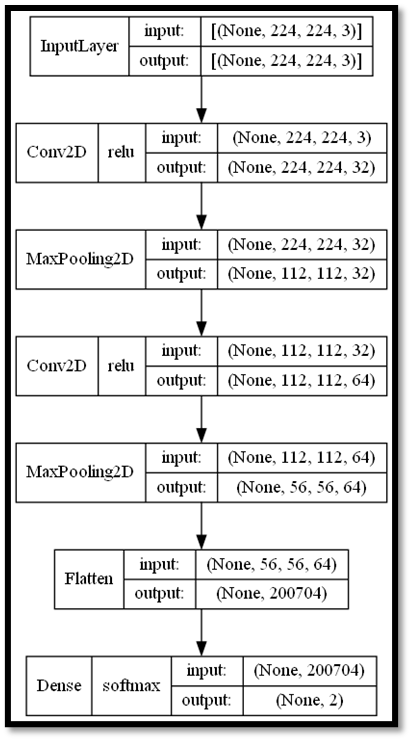
\includegraphics{assets/binaryClassificationArchitecture.png}}  
    \caption{The architecture of the proposed Binary Classification Neural Network}
    \label{binaryClassificationFigure}
\end{figure}

\newpage
I initially started with a simple intelligent algorithm to classify road images in two groups: roads that contain potholes and roads that do not contain potholes.
The proposed architecture (\ref{binaryClassificationFigure}) has two convolutional blocks (with 32 and 64 3x3 filters, respectively) followed by a dense layer with 2 neurons.
\begin{itemize}
	\item \textbf{Input:} A 224x224 image (\ref{binaryClassificationExamples})
	\item \textbf{Output:} 1 or 0 (there are potholes in the image or not).
\end{itemize}

\begin{figure}[htbp]
    \centerline{\includegraphics{assets/binaryClassificationExamples.png}}  
    \caption{Input examples}
    \label{binaryClassificationExamples}
\end{figure}

\newpage
I tested the algorithm on 70 test images and I obtained the following confusion matrix (\ref{binaryClassificationCM}):

\begin{figure}[htbp]
    \centerline{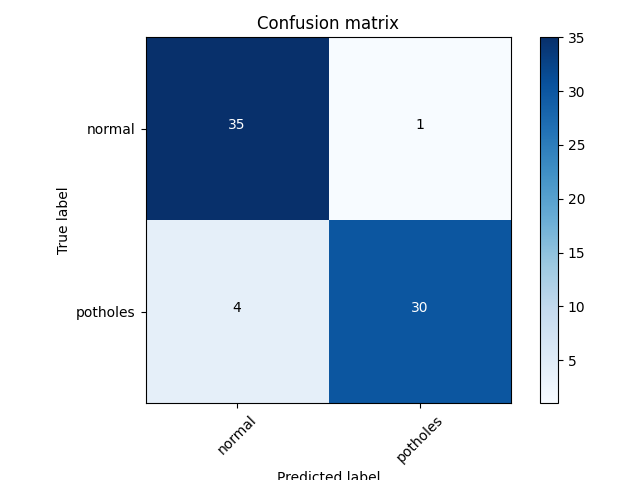
\includegraphics{assets/binaryClassificationCM.png}}  
    \caption{Confusion matrix obtained from testing my Binary Classification Neural Network}
    \label{binaryClassificationCM}
\end{figure}

\newpage
\section{UNet Neural Network}
\label{section:uNet}

\begin{figure}[htbp]
    \centerline{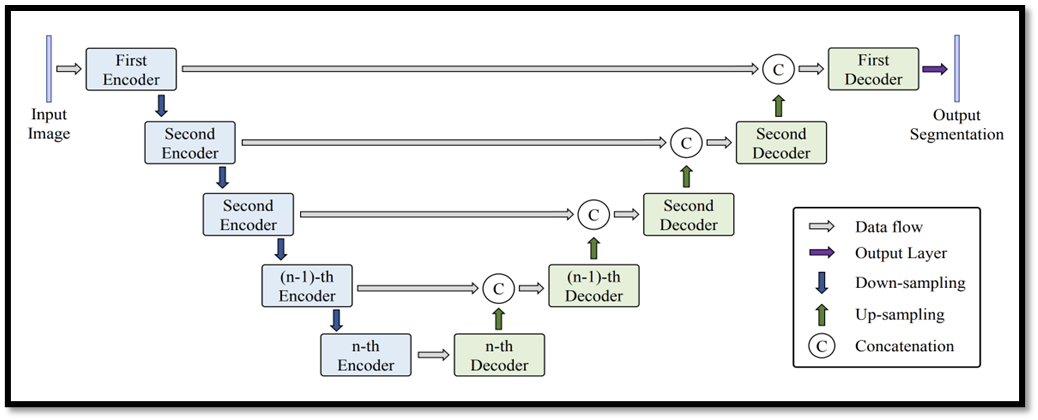
\includegraphics{assets/uNetArchitecture.png}}  
    \caption{The architecture of the proposed UNet architecture}
    \label{uNetArchitecture}
\end{figure}

I then began working on an UNet Neural Network to predict a mask over the potholes area in the image. The proposed architecture is presented in the figure \ref{uNetArchitecture}.
\begin{itemize}
	\item \textbf{Input:} A 400x400 image (\ref{uNetExamples})
	\item \textbf{Output:} Black and white image representing the mask (\ref{uNetExamples})
\end{itemize}

\begin{figure}[htbp]
    \centerline{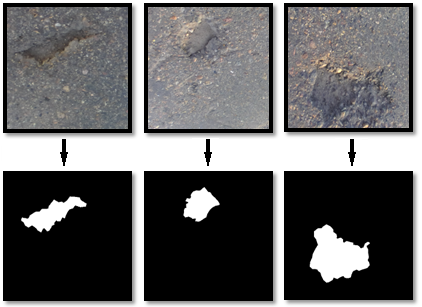
\includegraphics{assets/uNetExamples.png}}  
    \caption{Input-Output examples}
    \label{uNetExamples}
\end{figure}

\newpage
\section{AA-UNet Neural Network}
\label{section:uNet}

\begin{figure}[htbp]
    \centerline{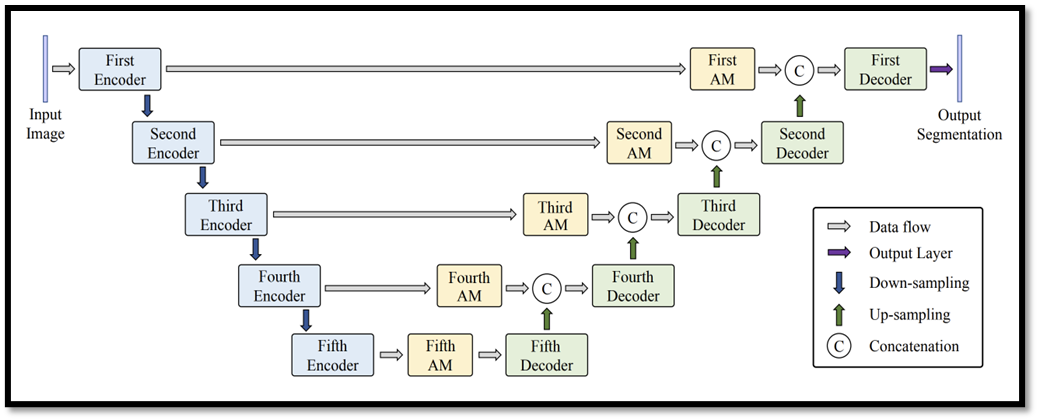
\includegraphics{assets/aAUNetArchitecture.png}}  
    \caption{The architecture of the proposed AA-UNet architecture}
    \label{aAUNetArchitecture}
\end{figure}

Ultimately, I began working on an AA-UNet Neural Network to predict a mask over the potholes area in the image. In addition to the previous UNet architecture (\ref{uNetArchitecture}), the proposed architecture (\ref{aAUNetArchitecture}) has three  types of attention modules (\ref{aAUNetAttentionModules}) used on each of the five levels before concatenation.

\begin{figure}[htbp]
    \centerline{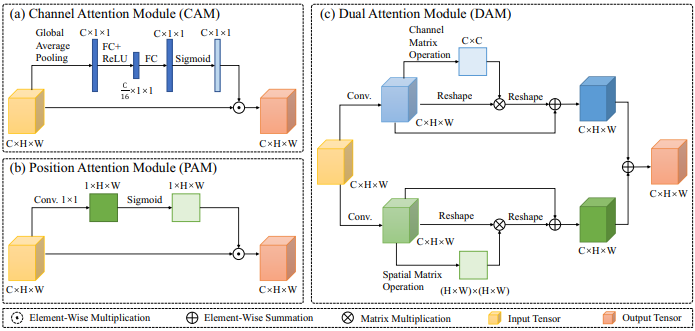
\includegraphics{assets/aAUNetAttentionModules.png}}  
    \caption{The three attention modules that I used}
    \label{aAUNetAttentionModules}
\end{figure}

\newpage
\begin{itemize}
	\item \textbf{Input:} A 400x400 image (\ref{uNetExamples})
	\item \textbf{Output:} Black and white image representing the mask (\ref{uNetExamples})
\end{itemize}

\begin{figure}[htbp]
    \centerline{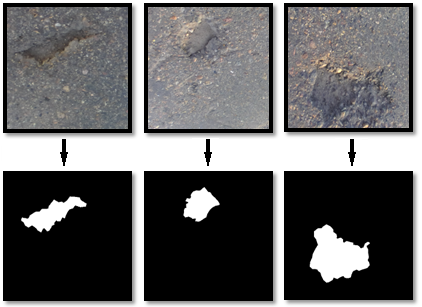
\includegraphics{assets/uNetExamples.png}}  
    \caption{Input-Output examples}
    \label{uNetExamples}
\end{figure}


\newpage
\chapter{Application}
\label{chapter:application}

\section{Numerical validation}
\label{section:numericalValidation}

\subsection{Results}
\label{section:results}

The UNet and AA-UNet networks were tested on 180 test images, and the results are represented in the following table (\ref{uNetEval}):

\begin{figure}[htbp]
    \centerline{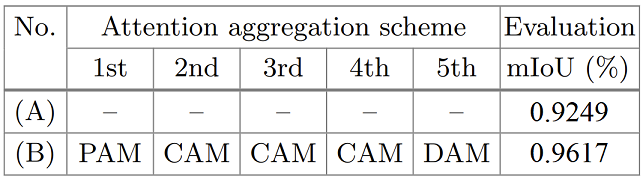
\includegraphics{assets/uNetEval.png}}  
    \caption{Performance evaluation of the UNet and AA-UNet networks}
    \label{uNetEval}
\end{figure}


\bibliographystyle{plain}
\bibliography{BibAll}

\end{document}
